\documentclass[../main.tex]{subfiles}
\graphicspath{{\subfix{../images/}}}



\begin{document}

\subsection{Product perspective}
% Include scenarios and further details on the shared phenomena and a domain model (class diagrams and state diagrams)

\subsubsection{Scenarios}
\textbf{A. Driver wants to start to use the system}
\vspace{-0.7em}
\\
\\
Driver A owns an electric vehicle, but he always has troubles on choosing which charging stations to go to charge his car. He decides to start to use the eMall platform. First, he downloads the application and then registers himself with the requested data. After the completion, he logs into his account. He registers his vehicle in the profile and finally he can take advantage of all the services offered by the application.
\vspace{2em}
\\
\\
\textbf{B. Driver wants to get information about charging stations}
\vspace{-0.7em}
\\
\\
Driver D arrives in a new city for business, and he wants to compare the price of charging stations with those in his city. For this reason he decides to use the eMall application. After he logs in with his account, the map in the main page shows the position of Driver D and the available charging stations nearby. When Driver D selects a charging station from the map, he can visualize its charging prices and the special offers if available.
\vspace{2em}
\\
\\
\textbf{C. Driver wants to book a charge}
\vspace{-0.7em}
\\
\\
Driver E realises that his electric vehicle is running out of battery, and he decides to use the eMall platform to find the nearest charging station. He does the login and successfully enters into his account. Then he clicks on the “List” button to visualize a list of charging stations sorted by the distance. He chooses the nearest charging station and books the charge selecting the earliest time frame available. 
\vspace{2em}
\\
\\
\textbf{D. Driver starts the charging process at the station}
\vspace{-0.7em}
\\
\\
Driver Z has already booked a charge on the eMall platform. He arrives at the chosen charging station by time, and he successfully authenticates at the charging column through the code shown on his mobile application. Then he plugs the vehicle in, and the display of the charging column shows him the remaining charging time. Now the car is locked there, and Driver Z is free to go to deal with personal issues while leaving the car at the charging station.
\vspace{2em}
\\
\\
\textbf{E. Driver receives suggestions about going to charge the vehicle}
\vspace{-0.7em}
\\
\\
The eMall system checks the status of the battery and the schedule of Driver Y when he begins his journey. The sensor detects the low battery state of the vehicle, and the system is notified about this condition. After checking the calendar and the navigation system of the driver, the system notices that he will arrive nearby a certain charging station with available charging sockets. At this point Driver Y receives a notification on his smartphone with the suggestion to go at that charging station and charge the vehicle. The charging station's location is reported too.
\vspace{2em}
\\
\\
\textbf{F. Operator wants to check the status of the charging station}
\vspace{-0.7em}
\\
\\
Operator X wants to check the status of the charging station managed by him. He logs into his operator account, and then he visualizes the status page of the charging station: the information shown includes its location, its external status (number of charging sockets available, their type, their cost, the special offers, and the estimated time until finishing the charge), and its internal status (the amount of energy available in its batteries, number of vehicles being charged, the time left and the amount of power absorbed).
\vspace{2em}
\\
\\
\textbf{G. Operator wants define a special offer}
\vspace{-0.7em}
\\
\\
Operator W wants to promote a special offer in the charging station managed by him. He logs into his operator account, and selects the option to manage the charging offers for that station. He decides a new cost for a certain charging type, with the starting date and the end date, and he confirms the modification. Now the system displays this offer on the charging station page.
\vspace{2em}
\\
\\
\textbf{H. Operator wants to acquire energy}
\vspace{-0.7em}
\\
\\
Operator V manages a charging station, and he wants to acquire energy for it. He logs into his operator account, and he checks the list of the current prices of energy published by the Distribution System Operators. After thinking on the options, the operator V decides from which DSO he would like to acquire energy, and select it from the list. He is asked to input the quantity of energy he wants to acquire, and the system shows the summary of his operation. After confirming, the request of the operator will be sent to the chosen DSO and processed soon. 
\vspace{2em}
\\
\\
\textbf{I. Operator wants to decide the energy source for charging}
\vspace{-0.7em}
\\
\\
Operator U wants to manually decide where to get energy for the charging station. He logs into his operator account, and he visualizes the current schedule in the main page of the charging station: the energy source is determined dynamically unless any human operator decides to change it. Operator U selects one of the available alternatives from the list displayed by the system, and the change is applied after his confirmation. 
\vspace{2em}


% \begin{enumerate}
%     \item User wants to start using the system
%     \item User wants to get information about the charging stations
%     \item User wants to book a charge
%     \item User starts the charging process at the station
%     \item Operator wants to check the status of the charging station
%     \item Operator wants to define a special offer
%     \item Operator wants to acquire energy
%     \item Operator wants to decide where to get energy for charging
% \end{enumerate}

\newpage
\subsubsection{Class Diagram}
The class diagram of the system shows the relevant entities and their relations. 
\begin{figure}[H]
    \centering
    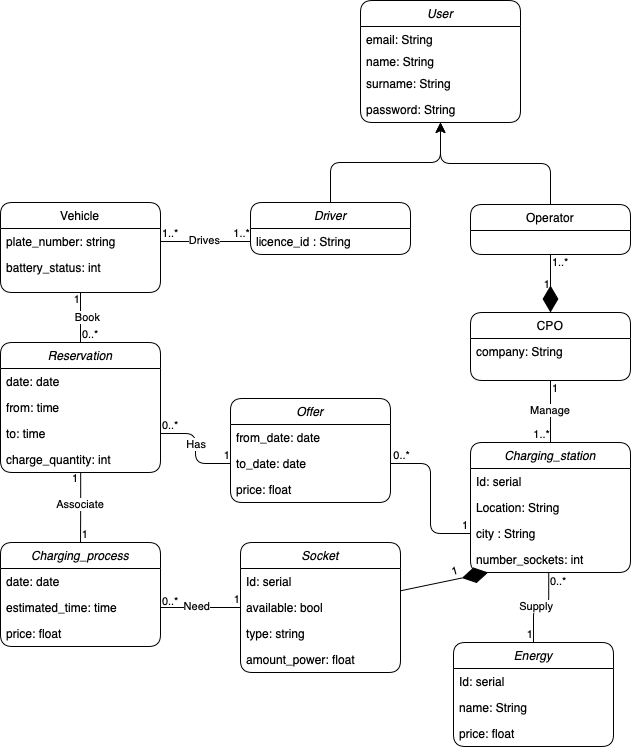
\includegraphics[width=0.85\textwidth]{images/classDiagram.png}
    \caption{Class Diagram representing the system}
    \label{fig:class}
\end{figure}


\subsubsection{Statecharts}
The state diagrams presented in this part have the objective to better represent some events of the system by defining the state transitions. 

\begin{figure}[H]
    \centering
    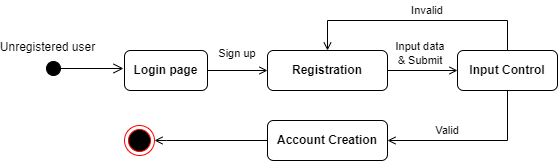
\includegraphics[width=0.9\textwidth]{statecharts/sc_register.png}
    \caption{State diagram of the registration process. When the operation is completed, the user is redirected to the Login page.}
    \label{fig:register}
\end{figure}

\begin{figure}[H]
    \centering
    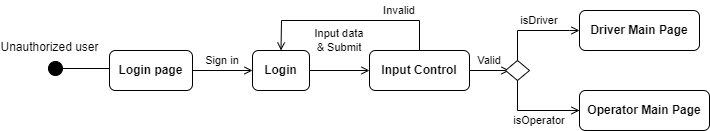
\includegraphics[width=0.95\textwidth]{statecharts/sc_login.png}
    \caption{State diagram of the login process. If the authentication is successful, the user is redirected to the corresponding Main page with respect to his role (driver or operator). }
    \label{fig:login}
\end{figure}

\begin{figure}[H]
    \centering
    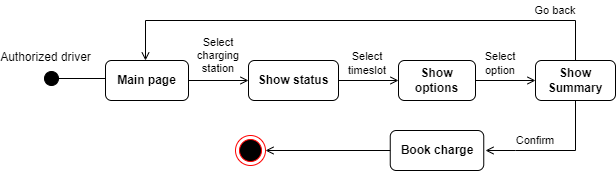
\includegraphics[width=0.95\textwidth]{statecharts/sc_bookCharge.png}
    \caption{State diagram of the booking process. The authorized driver has already logged in, and he wants to book a charge. He is asked to choose the charging station, the time slot and the charging options respectively. After the completion of the process, the driver is redirected to the Main page and he can visualize the reservation in his profile.}
    \label{fig:bookCharge}
\end{figure}

\begin{figure}[H]
    \centering
    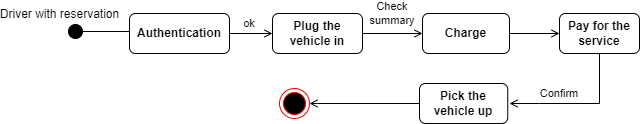
\includegraphics[width=0.95\textwidth]{statecharts/sc_charge.png}
    \caption{State diagram of the charging process. The driver has booked a time slot for charging, and he arrives at the charging station. He authenticates at the charging column, and plugs the vehicle in to start charging. When the operation is done, the driver is asked to pay for the charge before picking up the vehicle.}
    \label{fig:charge}
\end{figure}

\begin{figure}[H]
    \centering
    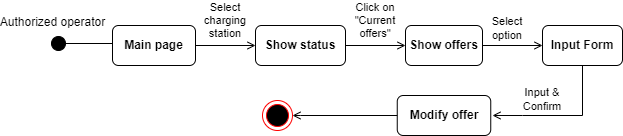
\includegraphics[width=0.95\textwidth]{statecharts/sc_modifyOffer.png}
    \caption{State diagram about promoting a new offer for the charging station. The authorized operator is asked to choose the charging station and to set the offer's price, starting and end date. At the end of the process, the operator is redirected to the Main page.}
    \label{fig:modifyOffer}
\end{figure}

\begin{figure}[H]
    \centering
    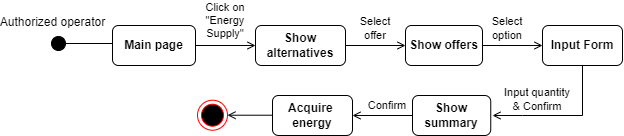
\includegraphics[width=0.95\textwidth]{statecharts/sc_acquireEnergy.png}
    \caption{State diagram of the energy acquisition process. The authorized operator visualizes the offers published by the DSOs, and submits an energy acquisition request with the required data.}
    \label{fig:acquireEnergy}
\end{figure}

\begin{figure}[H]
    \centering
    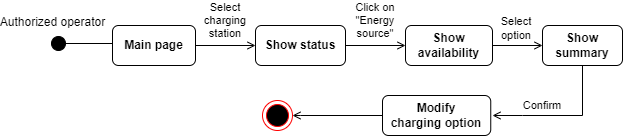
\includegraphics[width=0.95\textwidth]{statecharts/sc_changeChargeOption.png}
    \caption{State diagram about changing the energy source for the charges. The operator has logged in and he checks the availability of energy sources of the charging station. He then chooses the option to modify the charging sources in use.}
    \label{fig:changeChargeOption}
\end{figure}



\subsection{Product functions}
% Summary of most important requirements
In this section, a detailed description of the main functionalities of eMall is reported.
\\
\\
\textbf{A. Give information about the charging stations to users}
\vspace{-0.7em}
\\
\\
Giving information about the charging stations is at the basis of the system, and the given information is different according to the type of user.
\\
\\
The system will show to the drivers the location of nearby charging stations, their cost and eventually the available special offers. The drivers will know the number and type of available charging sockets in the chosen station, if all sockets of the chosen type are occupied, and the system will also show the estimated amount of time to have it be freed. 
\\
\\
On the other hand, the system will show to the operators the status of their charging station, such as the amount of energy available in its batteries, the number of vehicles being charged, the amount of power absorbed by these vehicles and the time left to finish the charge.
\vspace{1.5em}
\\
\\
\textbf{B. Book a charge}
\vspace{-0.7em}
\\
\\
The system will offer to the drivers the possibility to book a charge at a chosen charging station. This functionality will help them to avoid long queue of people waiting for a charging socket, and to better organize their schedule. 
\\
\\
The system will present to the drivers the charging stations and their sockets’ available timeframe. If the driver confirms a book, the system will reserve that socket in that timeframe. 
\vspace{1.5em}
\\
\\
\textbf{C. Charge a vehicle}
\vspace{-0.7em}
\\
\\
Allowing to charge a vehicle is one of the most important functionalities of the system. Thanks to the interaction between eMSPs and CPOs, the system will start a charging process at a certain station according to the amount of power supplied by the socket. The process will also be monitored by the system to infer when the battery is full. When the process is finished, the system will notify the driver.
\vspace{1.5em}
\\
\\
\textbf{D. Suggest the users to charge the vehicle}
\vspace{-0.7em}
\\
\\
The system will be able to suggest the driver to charge the vehicle actively, according to some monitored aspects. For example, checking the status of the vehicle’s battery allows the system to notify the driver when the battery level is low. The system will also recommend some special offers of charging stations after checking the availability of the charging slots at these stations.
\\
\\
If the driver gives consent, the system will provide the possibility to make suggestions refer to the driver’s schedule, by getting access to his/her calendar and navigation system.
\\
\\
This functionality can remind the driver of charging the vehicle without introducing much interference to his daily routine.
\vspace{1.5em}
\\
\\
\textbf{E. Manage the charging station}
\vspace{-0.7em}
\\
\\
An important aspect of the system is to help the CPOs to manage the owned charging stations.
\\
\\
A charging station needs to acquire energy from external DSOs. So it is important to decide when, how much and from which DSO to acquire energy. The system will be able to make these decisions in an autonomous way by checking the availability of the DSOs and the current energy information acquired by them.
\\
\\
Moreover, the system will offer the functionality to dynamically decide the cost of a charge and set special offers based on the previous information. And when a vehicle starts charging, the system will monitor the process and decide dynamically where to get energy for the charge, such as from station battery, DSO or a mix thereof according to availability and cost. 
\\
\\
All these kinds of decision could be made by the system automatically, but it will also provide the possibility to the human operators to handle each option.


\subsection{User characteristics}
% Include anything that is relevant to clarify their needs
There are three types of actors that we consider in the eMall system:
\begin{enumerate}
    \item \textbf{Unregistered user} \\
        An electric vehicle’s driver that cannot use eMall’s functionalities without registering to the eMall platform.
    \item \textbf{Driver} \\
        An electric vehicle’s driver, registered to the platform, who can use the system to find charging stations and charge his/her electric vehicles, to book charges and to receive suggestions.
    \item \textbf{Operator} \\
        A registered user who works for a specific CPO. The Operator can use the system to manage the charge stations of the belonged CPO and to receive current energy information from DSOs.
\end{enumerate}




\subsection{Assumption, dependencies and constraints}
% Include domain assumptions
% Anything that will limit the developer's options (e.g. regulations, reliability, criticality, hardware limitations, parallelism, etc.)


\subsubsection{Domain assumptions}
\begin{center}
\begin{longtable}{| c | p{12cm} | } 
\hline
\textbf{Identifier} & \textbf{Description} \\
\hline
% D1 & There exists APIs that retrieve correct information about Drivers’s daily schedule and his navigation system \\ 
% \hline
D1 & Each electric vehicle has an unique number plate for identification \\
\hline
D2 & Drivers will go to charge in the charging station indicated by their reservation\\
\hline
D3 & Drivers will arrive at the chosen charging station in time for the reservation \\
\hline
D4 & Drivers will complete the charging process within the booked time slot \\
\hline
D5 & Drivers makes a significant use of their calendar \\
\hline
% D5 & Driver cannot book a time slot before the current time \\
% we need to implement this, so its not a domain assumption
D6 & Drivers actually pay for the obtained service \\
\hline
% D7 & The information offered by CPMSs is reliable
%  \\
% \hline
D7 & The information offered by the external DSOs is reliable \\
\hline
D8 & The charging stations work correctly \\
\hline
D9 & The geolocation obtained from external API is reliable \\
\hline
D10 & Drivers own a valid driving licence \\
\hline
\end{longtable}
\end{center}

\subsubsection{Constraints}
\begin{center}
\begin{longtable}{| c | p{12cm} | } 
\hline
\textbf{Identifier} & \textbf{Description} \\
\hline
C1 & The permission of acquiring personal data (e.g. calendar and navigation system) must be given by the driver \\
\hline
C2 & Users have a device with properly working internet connection \\
\hline
\end{longtable}
\end{center}












\end{document}
